\documentclass[aspectratio=169]{beamer}
\usetheme{Boadilla}
\usecolortheme{whale}
\usepackage[utf8]{inputenc}
\usepackage[spanish,es-nodecimaldot]{babel}
\usepackage{amsmath}
\usepackage{amsfonts}
\usepackage{amssymb}
\usepackage{graphicx}
\graphicspath{{./figures/}}
\usepackage{ragged2e}
\usepackage{xcolor}
% \usepackage{listings}
\usepackage[outputdir={E:/tmp}]{minted}
% \usepackage[outputdir={/home/espinosa/tmp}]{minted}
\setminted[latex]{xleftmargin=1cm}
\usepackage{biblatex}
\addbibresource{bib.bib}
\setbeamercolor{bibliography entry title}{fg=blue!50!cyan}
\setbeamercolor{bibliography entry author}{fg=violet}
\setbeamercolor{bibliography entry location}{fg=green}
\setbeamercolor{bibliography entry note}{fg=orange}
\setbeamerfont{bibliography entry title}{size=\footnotesize,series=\bfseries}
\setbeamerfont{bibliography entry author}{size=\small}
\setbeamerfont{bibliography entry location}{size=\small}
\setbeamerfont{bibliography entry note}{size=\tiny}
\usepackage{hyperref}
\hypersetup{
  colorlinks=true,
  linkcolor=cyan,
  filecolor=magenta,
  urlcolor=cyan,
}
\setbeamertemplate{navigation symbols}{}
\setbeamertemplate{caption}[numbered]
\definecolor{lightgrey}{rgb}{0.9,0.9,0.9}
\definecolor{darkgreen}{rgb}{0,0.6,0}
\definecolor{codegray}{rgb}{0.5,0.5,0.5}
\renewcommand{\listingscaption}{Código}
\newminted{latex}{
            frame=lines,
            framesep=2mm,
            baselinestretch=1.2,
            bgcolor=\color{lightgrey},
            fontsize=\footnotesize,
            linenos
}
% \lstset{language=[LaTeX]TeX,
%         texcsstyle=*\bf\color{blue},
%         frame=single,
%         numbers=left,
%         numberstyle=\tiny\color{codegray},
%         numbersep=5pt,
%         breaklines=true,
%         keywordstyle=\color{darkgreen},
%         literate=*{\{} {{\textcolor{darkgreen}\{}}{1}%
% 			         {\}} {{\textcolor{darkgreen}\}}}{1}%
% 			         {[} {{\textcolor{darkgreen}[}}{1}%
% 			         {]} {{\textcolor{darkgreen}]}}{1}%
% 			         {\$} {{\textcolor{darkgreen}\$}}{1},
%         commentstyle=\color{red},
%         frame=none,
%         tabsize=2,
%         backgroundcolor=\color{lightgrey},
%         captionpos=b,
% }
\title{Introducción a \LaTeX}
\subtitle{\textit{Crash Course}}
\author[Carlos Espinosa]{Dr. Carlos Crispín Espinosa Ponce}
\institute[FC-UNAM]{Facultad de Ciencias\\Universidad Nacional Autónoma de México}
\date{5 de agosto}

\begin{document}
  \begin{frame}
    \maketitle
  \end{frame}
  \section{Introducción}
    \begin{frame}[allowframebreaks]
      \frametitle{Referencias}
      \printbibliography
      \nocite{*}
    \end{frame}
    \begin{frame}
      \frametitle{¿\LaTeX?}
      \begin{center}
        
\includegraphics[scale=0.4]{latex_meme}
      \end{center}
    \end{frame}
    \subsection{Latex y sus características}
      \begin{frame}
        \frametitle{¿Qué es \LaTeX?}
        \onslide<1,2,3>{
          \begin{exampleblock}{\LaTeX}
            \justifying
            Es un \emph{markup language} para la escritura de documentos de alta calidad. Su principal característica es poder manejar el contenido y el formato de manera independiente.
          \end{exampleblock}
        }
        \onslide<2,3>{
          \begin{alertblock}{Procesadores de texto convencionales}
            \justifying
            Los procesadores de texto como \emph{Microsoft Word} o \emph{LibreOffice} siguen la filosofia \textbf{WYSIWYM} (What You See Is What You Mean).
            Esto quiere decir que el formato que tenga el documento será el mismo que obtendremos cuando sea impreso.
          \end{alertblock} 
        }
        \onslide<3>{
          \LaTeX\ es \emph{gratis} y \textbf{open source} lo que ha permitido su mejora continua por más de 30 años, contando con una gran cantidad de \emph{plantillas} y \textbf{paquetes}.
        }
      \end{frame}
      \begin{frame}
        \frametitle{¿Por qué aprender \LaTeX?}
        \justifying
        \onslide<1,2,3>{
          \LaTeX\ es especialmente popular entre científicos dada su versatilidad y practicidad. Presenta diversar ventajas ante un procesador de texto convencional.
        }
        \onslide<2,3>{
          \begin{itemize}
            \item Manejo por separado del contenido y el formato.
            \item Personalización y creación de comandos
            \item Los archivos se guardan en archivos de \emph{texto plano}
              \begin{itemize}
                \item Se puede editar en ``cualquier editor'' 
                \item Estructura fácilmente reconocible
                \item Automatización de procesos
                \item Posible uso de programas de \textbf{gestión de versiones}
              \end{itemize}
            \item Documentos portables entre diferentes sistemas operativos.
          \end{itemize} 
        }
        \onslide<3>{
          A pesar de sus ventajas ante un procesador de texto convencional, \LaTeX\ puede tener una complicada curva de aprendizaje.
        }
      \end{frame}
    \subsection{Trabajando con LaTeX}
      \begin{frame}
        \frametitle{¿Qué necesitamos para trabajar en \LaTeX?}
        \justifying
        \onslide<1,2>{
          Para poder crear un documento en \LaTeX\ podemos trabajar de dos maneras:
          \begin{itemize}
            \item \textbf{Tradicional}: Instalación local en nuestra computadora.
            \item \textbf{Online}: No se necesita instalación, solamente una conexión de internet.
          \end{itemize}
        }
        \onslide<2>{
          Independiente al método que usemos, se necesitan dos (o tal vez tres) cosas fundamentales:
          \begin{itemize}
            \item \LaTeX\, el programa 
            \item Una serie de \emph{paquetes} básicos
            \item Editor y herramientas útiles
          \end{itemize}
        }
      \end{frame}
      \begin{frame}
        \frametitle{Trabajando de forma local} 
        \justifying
        \onslide<1,2>{
          Para trabajar de forma \textbf{local} en nuestra computadora tendremos que \textbf{instalar} una \emph{distribución} de \LaTeX. Aunque \LaTeX\ es \textbf{multi-plataforma}, existen diferentes distribuciones dependiendo del sistema operativo\footnote{Es buena idea revisar \href{https://www.latex-project.org/}{The LaTeX Project}}. 

        }
        \onslide<2>{
          Para los sistemas operativos más usuales tenemos:
          \begin{itemize}
            \item \textbf{Windows}: \href{https://www.tug.org/texlive/}{TeXLive}, \href{https://miktex.org/}{MiKTeX}
            \item \textbf{MacOS}: \href{https://www.tug.org/texlive/}{TeXLive}, \href{https://www.tug.org/mactex/}{MacTeX}
            \item \textbf{Linux}: \href{https://www.tug.org/texlive/}{TeXLive}
          \end{itemize}
        }
      \end{frame}
      \begin{frame}
        \justifying
        \frametitle{Trabajando en la nube\footnote{Recomendado}}
        Siguiendo las tendencias actuales, hay varias páginas que permiten poder crear documentos en \LaTeX\ sin la necesidad de instalar nada. Esto permite que, \emph{creando una cuenta}, se puedan crear documentos solamente con una conexión a internet y un dispositivo adecuado (computadora, tablet, \emph{smartphone}).

        A pesar de que hay muchos servicios hoy en día, el más utilizado actualmente es \href{https://www.overleaf.com/}{Overleaf}. Esta plataforma es usada por grandes colaboraciones científicas para realizar artículos de investigación. Igualmente es ampliamente usada por estudiantes para la creación de trabajos, reportes, tareas, tesis, etc. 
      \end{frame}
      \begin{frame}
        \frametitle{Herramientas para el trabajo en casa}
        \justifying
        \onslide<1,2>{
          Existen algunos editores especializados en \LaTeX\ que pueden hacer la edición un poco más sencilla. Estos editores pueden tener \textbf{autocompletado} de comandos, \textbf{menús interactivos}, correción de lenguaje, etc.

          Igualmente algunos editores \emph{clásicos} de edición de texto pueden servir con su respectiva configuración. 
        
        }
        \onslide<2>{
          Tenemos los editores de código:
          \begin{itemize}
            \item \href{https://www.xm1math.net/texmaker/}{TexMaker}
            \item \href{https://tug.org/texworks/}{TeXworks}
            \item \href{https://www.texstudio.org/}{TeXstudio}
          \end{itemize}

          Y los editores con filosofia WYSIWYG/WYSIWYM:
          \begin{itemize}
            \item \href{https://www.lyx.org/}{LyX}
            \item \href{https://www.texmacs.org/tmweb/home/welcome.en.html}{TeXmacs}
          \end{itemize}

          Igualmente editores de texto como \href{https://code.visualstudio.com/}{Visual Studio Code}, \href{https://www.sublimetext.com/}{Sublime Text}, \href{https://notepad-plus-plus.org/}{Notepad++} pueden ser útiles.
        }
      \end{frame}
  \section{Creando el primer documento}
    \subsection{Flujo de trabajo} 
      \begin{frame}
        \frametitle{¿Cómo trabaja \LaTeX?}
        \justifying
        \onslide<1,2>{
          Existen varios archivos importantes en el flujo de trabajo en un documento de \LaTeX. Entre ellos están los \textbf{archivos fuente}, \textbf{archivos de salida}, \textit{archivos de estilo y estructura}, \textit{archivos de fuentes}, \textit{archivos de formato}, etc.
        }
        \onslide<2>{

          \begin{center}
            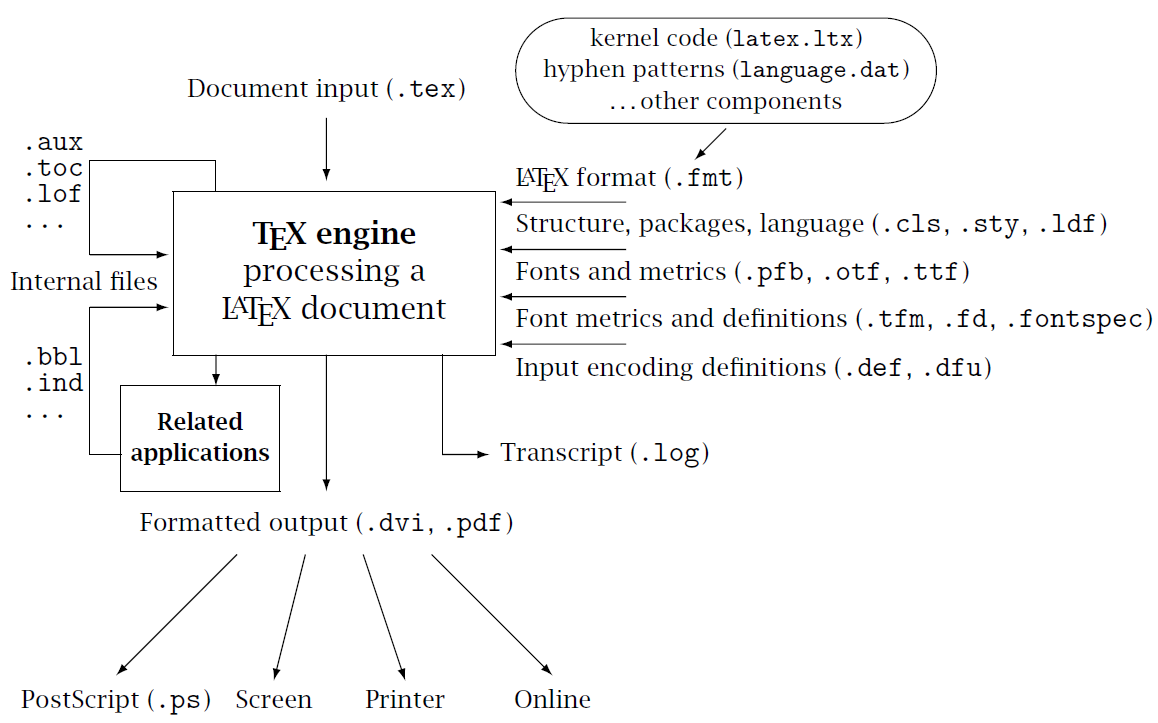
\includegraphics[width=0.55\textwidth]{latex_data_flow.png}
          \end{center}
        }
      \end{frame}
      \begin{frame}
        \frametitle{¿Qué son los archivos fuente?}
        \justifying
        \onslide<1,2,3>{
          El archivo más importante para crear un documento es un archivo fuente (\emph{source file}) que es un archivo de texto plano donde se entra el contenido, ecuaciones y comandos que serán procesados por \LaTeX.
        }
        \onslide<2,3>{

          \begin{block}{Archivo de texto plano}
            \justifying
            Es un archivo que contiene texto sin ningún tipo de formato. Dado que solo contienen caracteres, generalmente son ligero y se pueden abrir en cualquier sistema operativo.
          \end{block}
        }
        \onslide<3>{

          Nos encontraremos con los archivos fuentes en diversos ambítos fuera de \LaTeX, por ejemplo: en los lenguajes de programación.
        }
      \end{frame}
      \begin{frame}
        \frametitle{Archivos de salida}
        \justifying
        \onslide<1,2,3>{
          Los archivos de salida de \LaTeX\ es el documento final donde nuestro contenido ya tiene el formato deseado. En \LaTeX\ podemos identificar los siguientes tipos de \emph{archivos formateados}:
        }
        \onslide<2,3>{
          \begin{itemize}
            \item \textbf{dvi}: la representación propia de \LaTeX\ de un documento con formato. La precisión de las letras y posiciones es mejor que $0.01\,\mu\mathrm{m}$. Solo contiene los nombres y localizaciones de las fuentes y sus símbolos.
            \item \textbf{pdf}: El estándar de salida de \LaTeX\ hoy en día. Contiene toda la información para ``renderizar'' la información.
          \end{itemize}
        }
        \onslide<3>{
          \begin{alertblock}{Archivos auxiliares}
            \justifying
            Hay ciertos archivos \emph{internos} de \LaTeX\ que son utilizados para diversas acciones por ejemplo: referencias cruzadas, lista de figuras, etc. Estos archivos pueden borrarse tras la obtención del documento final.
          \end{alertblock}
        }
      \end{frame}
    \subsection{Hola Mundo en LaTeX}
      \begin{frame}[fragile]
        \frametitle{Creando (al fin) un documento en \LaTeX}
        En un archivo fuente vacío pondremos el siguiente código para crear un archivo simple con un mensaje:
        \begin{listing}[H] 
        \begin{minted}{latex}
\documentclass{article}
\begin{document}
Hola Mundo
\end{document}
        \end{minted}
          \caption{latex1.tex}
        \end{listing}
        Tenemos los dos comandos \textbf{fundamentales} de un documento de \LaTeX
        \begin{itemize}
          \item \mintinline{latex}{\documentclass}: Un archivo que será la base del documento entero. Provee varios estilo de formato y configuraciones por defecto.
          \item \mintinline{latex}{\begin{document}...\end{document}}: Usado para delimitar el \textbf{cuerpo} del documento. Al código que se encuentra entre \mintinline{latex}{\begin} y \mintinline{latex}{\end} se le llama \textbf{entorno} (\emph{environment}) 
        \end{itemize}
      \end{frame} 
      \begin{frame}[fragile]
        \frametitle{¿Y que tiene de especial \LaTeX?}
        En \LaTeX\ se prioriza la separación del contenido y el formato, por lo que podemos usar algunos \textbf{comandos} para que se le de formato automáticamente

        \begin{listing}[H] 
        \begin{minted}{latex}
\documentclass{article}
\author{John Doe}
\title{Documento prueba}
\begin{document}
\maketitle

Hola Mundo
\end{document}
        \end{minted}
          \caption{latex2.tex}
        \end{listing}
      \end{frame}
      \begin{frame}[fragile]
        \frametitle{Comandos extras/útiles}

        Algunos comandos básicos para empezar pueden ser:

          \begin{itemize}
            \item \mintinline{latex}{\date{\today}}
            \item \mintinline{latex}{\date{julio 2024}}
            \item \mintinline{latex}{\section{Título}}
            \item \mintinline{latex}{\subsection{Título}}
            \item \mintinline{latex}{\textbf{text}}
            \item \mintinline{latex}{\textit{text}}
            \item \mintinline{latex}{\backslash}: $\backslash$
            \item \mintinline{latex}{\{\}}: \{..\}
            \item \mintinline{latex}{\%}: \%
          \end{itemize}
          Los comentarios en \LaTeX\ se escriben con \%:

          \begin{minted}{tex}
\date{\today} %\date{Julio 2024}
          \end{minted}
      \end{frame}
    \subsection{Configurando el documento}
      \begin{frame}[fragile]
        \frametitle{Diferentes tipos de documentos} 
        El \textbf{comando} \mintinline{latex}{\documentclass} define el tipo y formato general del documento a crear. Existen diferentes tipos de documento:
        \begin{center}
			    \begin{tabular}{|c|c|}
			    \hline 
			    documentclass & Descripción \\ 
			    \hline 
			    article & \begin{tabular}{@{}c@{}}Clase para artículos científicos, presentaciones, \\ reportes cortos, 
			    
			    documentaciones de programas, invitaciones, etc\end{tabular}
			      \\ 
			    \hline 
			      proc & Documentos tipo \emph{expediente} basada en la clase \textit{article} \\ 
			    \hline 
			    report & \begin{tabular}{@{}c@{}} Documentos largos que contienen varios capítulos, \\ libros pequeños, tesis,etc 
    \end{tabular}
			     \\ 
			    \hline 
			    book & Clase para la escritura de libros \\ 
			    \hline 
			    slides & Clase para diapositivas\\ 
			    \hline 
			    memoir & \begin{tabular}{@{}c@{}}Basado en la clase book, con ella se puede\\ crear cualquier tipo de documento \end{tabular}
			    \\ 
			    \hline 
			    letter & Clase para la escritura de cartas en general \\ 
			    \hline 
			    beamer & Clase para la realización de presentaciones \\ 
			    \hline 
			    \end{tabular} 
        \end{center}
      \end{frame}
      \begin{frame}[fragile]
        \frametitle{Configuraciones extra}
        Podemos configurar algunas cosas desde el inicio del documento. El \textbf{comando} \mintinline{latex}{\documentclass} pose algunas opciones configurables.

        \begin{block}{Opciones en comandos de \LaTeX}
          En general, todos los comandos de \LaTeX\ tienen opciones configurables que pueden cambiarse con la siguiente \textit{sintáxis}

          \mintinline{latex}{\documentclass[opciones]{class}}
        \end{block}

        \begin{listing}[H] 
        \begin{minted}{latex}
\documentclass[11pt]{article}

\documentclass[letterpaper]{article}

\documentclass[landscape]{article}

\documentclass[twocolumn]{article}
        \end{minted}
        \end{listing}

      \end{frame}
  \section{Conclusiones}
    \begin{frame}
      \frametitle{Conclusiones}
        \LaTeX\ es un programa que nos permite crear documentos de alta calidad. Entre sus principales características están:
        \begin{itemize}
          \item Sigue una filosofia diferente a las paqueterias de ofimatica usuales.
          \item Se tiene una clara separación entre el contenido y el formato.
          \item Multiplataforma y versatilidad de uso.
          \item Software libre y con una comunidad que aporta funcionalidades en forma de \textbf{paquetes}.
        \end{itemize}
    \end{frame}
\end{document}
